\section{Preparación del entorno de trabajo}

La preparación del entorno de trabajo es una de las secciones que me hacen especial ilusión de este trabajo. Como decía Robert Owen, un reconocido empresario galés, en el siglo XVIII:

\begin{displayquote}
    Mejorando el entorno se mejora al hombre.
\end{displayquote}

El desarrollo de esta preparación previa ha supuesto un ahorro de tiempo bastante grande para el proyecto.
\\Esta sección irá estructurada en consonancia a la cronología de creación de cada parte del entorno. Empezamos por la semilla de todo: Github.

\subsection{GitHub}
Realizaremos la creación de nuestro proyecto en GitHub. Esto se hace de forma muy rápida y fácil.

\begin{enumerate}
    \item Nos dirigimos a la dirección de \url{github.com}
          \begin{figure}[htbp]
              \centering
              
\includegraphics[scale=0.3]{preparacion_entorno/pagina_principal_github.png}
              \caption{Página principal de GitHub}
          \end{figure}
    \item En la parte superior derecha nos aparece ``Sign up'' donde clicaremos y nos permitirá registrarnos dentro de la web.
    \item Una vez registrados volvemos a \url{github.com} y clicamos a la izquierda de ``Sign up'' que pone ``Sign in'' donde iniciaremos sesión.
    \item Cuando hayamos iniciado sesión nos dirigiremos a la parte superior izquierda y clicaremos en ``new'' para crear un nuevo repositorio.
    \item Rellenamos los campos que nos solicitan para crear un nuevo repositorio. Le damos el nombre de Inventarium y seleccionamos la opción para que el repositorio sea privado. También procedemos a añadirle un readme al archivo para poder describir partes del proyecto dentro de este. Por último pulsamos el botón ``Create repository''.
          \begin{figure}[htbp]
              \centering
              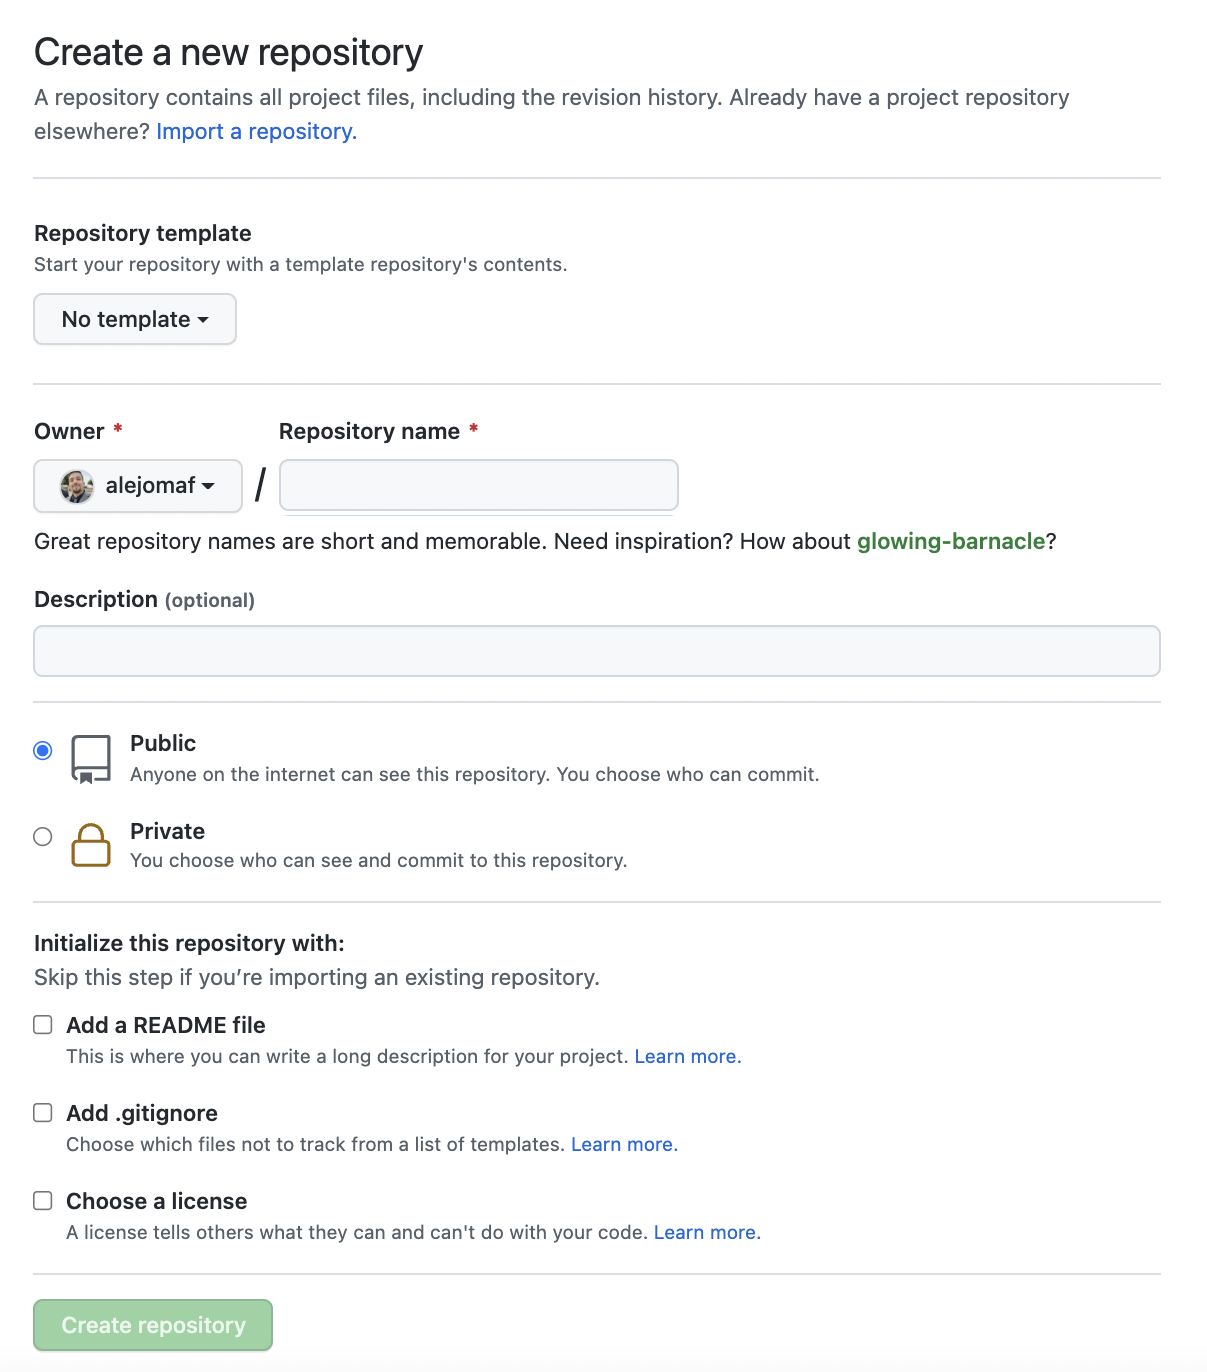
\includegraphics[scale=0.4]{preparacion_entorno/creando_nuevo_repositorio.png}
              \caption{Creando un nuevo repositorio dentro de GitHub}
          \end{figure}
\end{enumerate}

Con estos sencillos pasos ya tendríamos creado nuestro repositorio.

\subsection{Visual Studio Code y Google Cloud, los mejores amigos}
Hoy en día lo nuevo y a lo que nos dirigimos es la nube. Dentro de ella se pretenden que se realicen todos los procesos. La mayoría de herramientas y servicios que se nos ofrece hoy en día cumplen un modelo de caja negra. Es decir, interactuamos con él y recibimos respuestas pero no vemos qué procesos ocurren dentro de aquella cajita.
\\Por esta razón cada vez se empieza a disponer menos de un software como tal y se empiezan a pasar a servicios en línea. Esto no quiere decir que se dejen de usar programas o aplicaciones móviles. Pero la realidad es que sin internet; la mayoría no funcionaría.
\\Esto presenta desventajas siendo la principal que se depende constantemente de una conexión en línea que puede parecer que pasa en todos sitios pero en lugares remotos lejos de la ciudad como son los pueblos de montaña el internet no es el mejor compañero por decirlo de una manera. Por suerte este no es mi caso.
\\Las ventajas son enormes aunque solo nos centraremos en las que para mí implican mayor relevancia.
\\El tener ya un repositorio generado con nuestro proyecto subido dentro de él ya nos aporta bastante autonomía ya que podemos acceder a él y descargar nuestros datos desde cualquier lugar. Pero, ¿y configurarlo?
\\Aquí viene una problemática que no nos resuelve un entorno de repositorios. El tener que configurarlo todo cada vez que queremos trabajar desde un sitio distinto. Esto nos lo resuelven las máquinas virtuales en la nube. El generar un directorio de trabajo donde poder conectar nuestro Visual Studio Code y olvidarnos de preocupaciones.
\\Lo segundo que me parece más importante es el ahorro de memoria tanto de RAM como de disco y de procesos que se origina al hacer esto. No es lo mismo tener que trabajar con un portátil conectado todo el día a un enchufe que poder ir llevándotelo contigo durante todo el día por el escaso consumo de batería que tiene. Peor si es una torre, solo puedes trabajar desde un único sitio, con la problemática también de que siempre se te puede ir la luz, y más en una zona de pueblo de sierra como es la mía, suele ocurrir una vez cada dos semanas.
\\Estas ventajas expuesta son las que personalmente me favorecen a mí, pero ¿y si trabajara con un equipo? El poder tener varios compañeros de un mismo equipo trabajando en el mismo proyecto, tocando los distintos componentes que se están desarrollando dentro de tu aplicación es fantástico.

\subsubsection{Crear una máquina virtual en Google Cloud}
Los pasos para la creación de una máquina virtual son:

\begin{enumerate}
    \item El registro es fácil de realizar ya que la herramienta es propiedad de Google. Omitiremos este paso.
    \item Google Cloud se organiza mediante proyectos. Esto brinda facilidades a la hora de calcular el gasto que vamos a tener por el uso de la computación en la nube. Aparte de poder facilitar la búsqueda por cada proyecto que tengamos activo. Procederemos a crear un nuevo proyecto clicando arriba a la izquierda a la derecha del título de la página y posteriormente clicamos en nuevo proyecto.
    \item Luego desplegaremos la barra lateral de la izquierda y nos dirigiremos al apartado de Compute Engine.
    \item Clicamos en crear instancia. A la hora de rellenar los parámetros he comprobado que no hay que darle demasiada importancia a la zona o región donde se ubique nuestra máquina. Esta funciona a una velocidad bastante decente. En el apartado de configuración de máquina con 2GB de RAM y 1VCPU tendremos suficiente. El tamaño del disco eligiremos que sea de 20GB. Dentro de la sección Firewall habilitaremos el tráfico HTTP y HTTPS. Y pulsamos en crear.
    \item Después de haber creado la máquina le asignaremos una IP estática pública que la usaremos para conectarnos a ella mediante SSH.
    \item En el momento de haber creado la máquina esta nos ha dado una clave privada SSH para poder conectarnos a ella. La guardaremos.
\end{enumerate}

\subsubsection{Configurar claves SSH}

Teniendo ya la clave privada SSH de nuestra máquina virtual la utilizaremos para realizar la conexión a nuestra máquina. Pero para ello tenemos que configurarla. Accederemos al fichero usuario/.ssh/config y añadiremos tres nuevas líneas:
\begin{verbatim}
    Host "Aquí añadimos la dirección IP"
    HostName "Aquí ponemos el nombre del host"
    User "Aquí ponemos nuestro nombre de usuario"
\end{verbatim}
Lo último que nos queda es realizar la conexión mediante SSH a la máquina por Visual Studio Code.

\subsubsection{Realizar conexión SSH mediante Visual Studio Code}
Dentro del apartado de extensiones de Visual Studio Code buscaremos los siguientes plugins para instalar:

\begin{itemize}
    \item Remote - SSH
    \item Remote - SSH: Editing Configuration Files
\end{itemize}

Luego de la instalación de estas dos extensiones procederemos a realizar la conexión. Abajo a la izquierda nos aparecerá la opción de poder conectarnos mediante SSH. Clicamos y luego pulsamos en ``Connect to Host'' añadiendo la dirección IP estática pública que nos dio Google Cloud.
\\Ya tenemos la masa de nuestro entorno hecha, solo hace falta darle un poco de forma y calor para poder finalizarlo.

\subsection{Instalación de las extensiones de Visual Studio Code dentro de nuestra MV}

Esta es la lista de componentes con la que trabajaremos en todas las fases del proyecto. Accederemos a las extensiones dentro de Visual Studio Code y procedemos a instalarlas dentro de nuestra máquina virtual.

\begin{itemize}
    \item Docker
    \item LaTeX
    \item LaTeX Workshop
\end{itemize}

Los complementos de Latex nos ayudarán más tarde con la redacción del Trabajo de Fin de Grado.
\\En nuestro Visual Studio Code también instalaremos:

\begin{itemize}
    \item Bootstrap 4 snippets
    \item HTML snippets
    \item CSS snippets
\end{itemize}

\subsection{Configuración de nuestra máquina virtual}

Desde Visual Studio Code accederemos a la terminal de nuestra máquina virtual. Pinchamos en ``Ver'' en la sección superior y luego en Terminal. Desde ahí controlaremos a la máquina.

\subsubsection{Actualización del sistema}
Actualizaremos el sistema para evitar posibles fallos en un futuro:
\begin{verbatim}
    sudo apt-get update
    sudo apt-get upgrade
\end{verbatim}

\subsubsection{Instalación de Node JS}
\begin{verbatim}
    sudo apt install nodejs
\end{verbatim}

\subsubsection{Instalación de Angular 12}
\begin{verbatim}
    sudo npm install npm@latest -g
    sudo npm install -g @angular/cli
\end{verbatim}

\subsubsection{Instalación de Docker y Docker Compose}
\begin{verbatim}
    \\Instalacion de Docker

    sudo apt install apt-transport-https ca-certificates curl software-properties-common
    curl -fsSL https://download.docker.com/linux/ubuntu/gpg | sudo apt-key add -
    sudo add-apt-repository "deb [arch=amd64] https://download.docker.com/linux/ubuntu focal stable"
    sudo apt install docker-ce

    \\Instalacion de Docker Compose

    sudo curl -L "https://github.com/docker/compose/releases/download/1.26.0/docker-compose-$(uname -s)-$(uname -m)" -o /usr/local/bin/docker-compose
    sudo chmod +x /usr/local/bin/docker-compose
\end{verbatim}

\subsubsection{Configuración de credenciales de Git e instalación del repositorio}
\begin{verbatim}
    //Configuración de credenciales

    git config --global user.name "tu nombre de usuario"
    git config --global user.email "tu correo electrónico"
    git config --global user.password "tu contraseña"

    //El repositorio lo ubicaremos dentro de la carpeta raíz del usuario
    
    git clone https://github.com/alejomaf/Inventarium.git
\end{verbatim}